\subsection{Important definitions}

\begin{definition}
    For every $t \ge 0$, the $t$-thickening of the set $X$, denoted $X^t$, is
    the set of points of the ambient space with distance at most $t$ from $X$:
    $$X^t = \{y \in \R^n, \exists x \in X, ||x - y|| \le t\}.$$
    Equivalently, $X^t$ can be seen as a union of closed balls centered around
    every point of $X$.
\end{definition}

\begin{definition}[Hausdorff distance]
    Let $X$ be any subset of $\R^n$. The function distance to $X$ is the map 
    \begin{align*}
        \text{dist }(\cdot, X) : \R^n &\rightarrow \R \\
        y &\mapsto \text{dist }(y, X) = \inf\{||y - x||, x \in X\}
    \end{align*}
    A projection of $y \in \R^n$ on $X$ is a point $x \in X$ which attains
    this infimum. If such a point $x$ exists and is unique, we denote it
    $\text{proj }(y, X)$. 

    Then the Hausdorff distance cna be written as 
    $$
    d_H(X, Y) = \max(\sup_{y\in Y} \text{dist }(y, X), \sup_{x\in X} \text{dist }(x, Y))$$
\end{definition}

\begin{definition}
    Let $X$ be any subset of $\R^n$. The medial axis of $X$ is the subset
    $med(X) \subset \R^n$ which consists of points $y \in \R^n$ that admit at
    least two projections on $X$:
    $$
    med(X) = \{y \in \R^n, \exists x, x' \in X, x \neq x', ||y - x|| = ||y - x'|| = dist(y, X)\}
    .$$
\end{definition}

\begin{definition}
    Now, we define the reach of $X$ as its proximity from its medial axis:
    $$
    reach(X) = \inf\{dist(y, X), y \in med (X)\} = \inf\{||x - y||, x \in X, y \in med (X)\}
    $$
    Equivalently
    $$
    reach(X) = \sup\{t \ge 0, X^t \cap med (X) = \emptyset\}
    $$
\end{definition}

\begin{definition}
    Let $X$ be a topological space, and $U = \{U_i\}_{1\le i\le N}$ a cover of
    $X$. The nerve of $U$ is the simplicial complex with vertex set $\{1, ...,
    N\}$ and whose m-simplices are the subsets $\{i_1, ..., i_m\} \subset \{1,
    ..., N\}$ such that $\cap_{k=0}^m U_{i_k} \neq \emptyset$. It is denoted $\mathcal{N}(U)$.
\end{definition}

\begin{definition}
    Let $t \ge 0$ and consider the collection $\mathcal{V}^t = \{
    \bar{\B}(x,t), x \in X\}$. Its nerve is denoted Cech$^t(X)$ and is called the Cech complex of $X$ at time $t$.
\end{definition}

\begin{definition}
    Given a graph $G$, the corresponding clique complex is the simplicial
    complex whose vertices are the vertices of $G$, and whose simplices are
    the sets of vertices of the cliques of $G$. Some authors also call it the
    expansion of $G$
    .
\end{definition}

\begin{definition}
    The Rips complex of $X$ at time $t$ is the clique complex of the graph
    $G^t$ defined above. We denote it Rips$^t(X).$
\end{definition}

\subsection{Exercises}

\begin{exercise}
    Prove that, when $X$ is closed and bounded, a projection always exists. A set is bounded if there exists $R > 0$ such that $X \subset \B(R, 0)$.
\end{exercise}

\begin{proof}

Let $X$ a closed and bounded subset of $\R^n$. So it's compact by the
Heine-Borel theorem. The map $y \mapsto ||y - x||$ is continuos because for $y
\in \R^n$ and $\epsilon > 0$, if we take $\delta = \epsilon$, and $||y - w|| <
\delta, $
$$
\epsilon > ||y - w|| = ||(y - x) - (w - x)|| \ge |||y-x|| - ||w-x|||
$$

By the Weierstrass theorem, the function $y \mapsto ||y-x||$ has a global
minimum in $X$, that is, there exist $x^* \in X$ such that $||y - x^*|| \le
||y - x||, \forall x \in X$. So the infimum is well defined and a projection
always exist. However the uniqueness is not guaranteed.

\end{proof}

\noindent\linia

\begin{exercise}
    Let $||\cdot||+{\infty}$ be the sup norm of function $f : \R^n \to \R^m:
    ||f||_{\infty} = \sup_{x \in \R^n} ||f(x)||$. Prove that $d_H(X, Y) = ||\text{dist}(\cdot, X) - \text{dist}(\cdot, Y)||_{\infty}$.
\end{exercise}

\begin{proof}

We have that 
\begin{equation*}
    \begin{split}
        ||\text{dist }(\cdot, X) - \text{dist }(\cdot, Y)||_{\infty} &= \sup_{x \in \R^n} |\text{dist}(x, X) - \text{dist}(x, Y)| \\
        &\ge \sup_{x \in \R^n} (\text{dist}(x, X) - \text{dist}(x, Y)) \\
        &\ge sup_{y \in Y} dist(y,X)
    \end{split}
\end{equation*}
given that $Y \subset \R^n$ and $dist(y,Y) = 0$. Also

\begin{equation*}
    \begin{split}
        ||\text{dist }(\cdot, X) - \text{dist }(\cdot, Y)||_{\infty} &= \sup_{x \in \R^n} |\text{dist}(x, X) - \text{dist}(x, Y)| \\
        &\ge \sup_{x \in \R^n} (\text{dist}(x, Y) - \text{dist}(x, X)) \\
        &\ge sup_{x \in X} dist(x,Y)
    \end{split}
\end{equation*}
In special, $||\text{dist }(\cdot, X) - \text{dist }(\cdot, Y)||_{\infty} \ge
d_H(X,Y)$. 

The other inequality can be seen as follows. If $dist(x,Y) \le k, \forall x \in X$, then for all $w \in \R^n$ and $x \in
X$, $$dist(w,Y) \le dist(w,x) + dist(x,Y) \le dist(w,x) + k$$ and hence
$dist(w,Y) \le dist(w,X) + k$, taking the infimum. Likewise, if $dist(y,X) \le
k, \forall y \in Y$ we obtain $dist(w, X) \le dist(w,Y) + k$. Then 
$|dist(w,X) - dist(w,Y)| \le k$, for all $w \in \R^n$.
In particular $d_H(X,Y) \ge dist(x,Y), \forall x \in X$ and $d_H(X,Y) \ge
dist(y,X), \forall y \in Y$. By the fact we have proved 
$$
d_H(X,Y) \ge \sup_{w \in R^n}|dist(w,X) - dist(w,Y)| = ||dist(\cdot, X) - dist(\cdot, Y)||_{\infty}
$$
We conclude $d_H(X,Y) = ||dist(\cdot, X) - dist(\cdot, Y)||_{\infty}$. 

\end{proof}

\noindent\linia

\begin{exercise}
    Let $X, Y$ be two closed and bounded subsets of $\R^n$. Show that for
    every $t \ge 0$, the thickenings satisfy 
    $$
    d_H(X^t, Y^t) \le d_H(X, Y).
    $$ 
    Give an example for which $d_H(X^t, Y^t) < d_H(X, Y)$.
\end{exercise}

\begin{proof}

Let's do it by steps, because dealing with infimum and supremum can be trick.
Let $t \ge 0$ and denote $dist$ by $d$. 

\begin{enumerate}
    \item Let's prove $d(w,Y^t) \le d(w,Y) - t, \forall w \in X^t/Y^t$. 
    
    Take $y \in Y$ and denote $\beta = ||w - y|| > t$. Take the point $\alpha
    w + (1 - \alpha)y$ such that, for some $\alpha \in [0,1]$, $t = ||\alpha y
    + (1-\alpha)y - y|| = \alpha\beta$, that is, $\alpha = t/\beta < 1$. So we
    will have $||w - \alpha w - (1 - \alpha)y|| = (1 - \alpha)\beta = \beta -
    t$. It implies $d(w,Y^t) \le d(w,Y) - t$. After we will see the restriction
    over the domain of $w$ is not restrictive. 

    \item  $\sup_{w \in X^t} d(w, Y) \le \sup_{x \in X} d(x,Y) + t$ 
    
    If $w \in X^t$, there exists $x \in X$ such that $||w - x|| \le t$.
    So $d(w, Y) \le d(x,Y) + t \le \sup_{x \in X} d(x,Y) + t$. It values for
    all $w$, then $\sup_{w \in X^t} d(w, Y) \le \sup_{x \in X} d(x,Y) + t$. 

    \item $\sup_{w \in X^t} d(w, Y^t) \le \sup_{x \in X} d(x, Y)$. 
    
    For every $w \in X^t/Y^t$,  we have $d(w, Y^t) \le \sup_{w \in X^t} d(w, Y) -
    t$, because of what we've proved on point 1. Then 
    $$\sup_{w \in X^t/Y^t}
    d(w,Y^t) \le \sup_{w \in X^t} d(w, Y) -
    t \le \sup_{x \in X} d(x,Y),$$ as argued on point 2. Otherwise suppose $w
    \in Y^t \cap X^t$, then $d(w,Y^t) = 0$ and the inequality $\sup_{w \in X^t
    \cap Y^t} d(w, Y^t) = 0 \le \sup_{x \in X} d(x,Y)$ is trivial,
    because $d$ is a metric. Therefore 
    $$
    \sup_{w \in X^t} d(w, Y^t) = \max\{\sup_{w \in X^t
    \cap Y^t} d(w, Y^t), \sup_{w \in X^t/Y^t}
    d(w,Y^t)\} \le \sup_{x \in X} d(x,Y)
    $$

    \item We can show similarly that $\sup_{z \in Y^t} d(z, X^t) \le \sup_{y
    \in Y} d(y, X)$. 

    \item Therefore, the last two points imply $d_H(X^t, Y^t) \le d_H(X,Y)$. 

\end{enumerate}

\textbf{Example}

Consider the following construction. Let $C_0$ be the origen and $C_i$ be the
circumference of center 0 and radius $\sum_{j=0}^{i-1} 2^{-j} = 2 - 2^{1-i}$.
Each time the adicional value to the radius of the next circle is decreasing
by half. All the circles are contained in $\B(0,2)$. We will define $$X =
\bigcup_{i=0}^{\infty} C_{2i} \text{ and } Y =
\bigcup_{i=0}^{\infty} C_{2i + 1}$$

\begin{figure}[H]
    \centering
    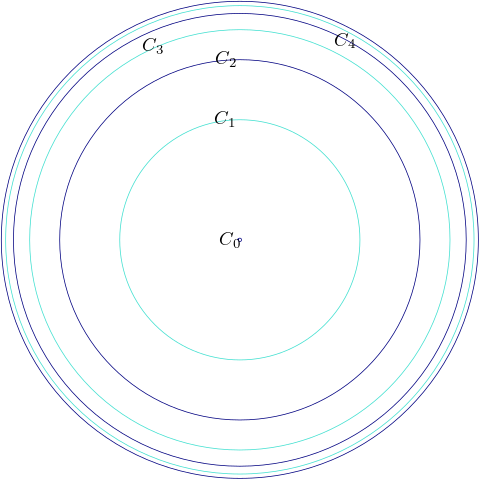
\includegraphics[width = 0.3\textwidth]{../images/circle-inside-circle.png}
\end{figure}

I claim that $d_H(X,Y) = 1$. For every $x \in C_i$, we have that $d(x,Y) =
2^{-i}$, because the closest point in $Y$ is in $C^{i+1}$. We can argue the
same for $d(y,X)$. Therefore $d_H(X,Y) = \sup_i 2^{-i} = 1$. Consider now
$X^t$ and $Y^t$ for some $t > 0$. We are creating rings with thickness $2t$.
Some rings of different sets are being joined. Let's calculate $d_H(X^t,
Y^t)$. In general, $d(x,Y^t)$ will decreased, be unaltered (when we pick some
point in a border of $C_i^t$ that maps to $C_{i+1}^t$ or go to $0$, when two
rings join. But it shall not increase. However if we take the origin, $d(0,Y)
= 1 - t$, but no other can have a greater distance. Thus, $d_H(X^t, Y^t) = 1-t
< 1 = d_H(X, Y)$. 

\end{proof}

\noindent\linia

\begin{exercise}
    Show that the Hausdorff distance is equal to
    $$inf\{t \ge 0, X \subset Y^t \text{ and } Y \subset X^t\}$$
\end{exercise}

\begin{proof}

Let $t$ such that $X \subset Y^t$ and $Y \subset X^t$. Take $x \in X$ and
consider $d(x,Y)$. By the choice of $t, x \in Y^t$, what implies $d(x,Y) \le
t$, because we can find $y \in Y$ such that $||x - y|| \le t$. As $x$ is
arbitrary, $\sup_{x \in X} d(x,Y) \le t$. The same can be told about $\sup_{y
\in Y} d(y, X)$. That implies $d_H(X,Y) \le t$. As we took arbitrary $t$,
applying the infimum we obtain 
$$d_H(X,Y) \le \inf\{t \ge 0, X \subset Y^t, Y \subset X^t\}.$$
Suppose the above inequality is strict ($<$). Then there is $\epsilon > 0$
such that $d_H(X, Y) + \epsilon$ is still less. Define $s = d_H(X,Y) + \epsilon$. Then $s > d(x,Y), \forall x \in X$ and $s > d(y,
X), \forall y \in Y$. As $s > d(x,Y)$, there is $y \in Y$ such that $||x - y||
< s \implies x \in \bar{\B}(x,y) \implies x \in Y^s$. This holds for every $x
\in X$, so $X \subset Y^s$. Likewise we prove $Y \subset X^s$. That is a
contradiction, since $s < \inf\{t \ge 0, X \subset Y^t, Y \subset X^t\}$. We
conclude that $d_H(X, Y) = \inf\{t \ge 0, X \subset Y^t, Y \subset X^t\}.$  

\end{proof}

\noindent\linia 

\begin{exercise}
    Compute the reach of the following subsets of $R^2$:
    \begin{enumerate}
        \item the set $\{(0, n), n \in \Z\},$
        \item the segment $\{(t, 0), t \in [0, 1]\},$
        \item the unit circle with origin $\sphere_1 \cup \{(0, 0)\}$,
        \item the square $\{(x, y) \in R^2, \max\{|x|, |y|\}  
        = 1\},$
        \item the ellipse $\{(x_1, x_2) \in \R^2, (\frac{x_1}{a})^2 +
        (\frac{x_2}{b})^2 = 1 \}$
    \end{enumerate}
\end{exercise}

\begin{proof}

\begin{enumerate}
    \item Define this set as $Z$. So $reach(Z) = \inf\{d(y,Z), y \in
    med(Z)\}$. We have that $med(Z) = \{(x,n+1/2), x \in \R, n \in \Z\}$, the
    bisector os two sequential points. For each point $y$ in one of these
    lines, $dist(y,Z) = ||(x,n+1/2) - (0,n)|| = ||(x,1/2)|| = \sqrt{x^2 +
    1/4}$. The infimum over $y$ occurs when $x = 0$ and we conclude $reach(Z)
    = 1/2$. 

    \item Denote this set as $I$. Take $y = (y_1, y_2) \in \R^2$. We want
    the values on $I$ which distance to $y$ is $d(y,I) = \inf\{\sqrt{(y_1 -
    t)^2 + y_2^2}, t \in [0,1] \} = \min\{\sqrt{(y_1 -
    t)^2 + y_2^2}, t \in [0,1] \}$, since $I$ is closed and bounded, there exists a projection. We must
    minimize $(y_1 - t)^2$ in the interval $[0,1]$, but this clearly have only
    one solution. We conclude $med(I) = \emptyset$ and $reach(I) = \infty$. 
    
    \item We have that $med(\sphere_1 \cap 0) = \partial\B(0,1/2)$. For each
    $y \in \partial\B(0,1/2), d(y,Z) = 1/2$, the distance to the origin.
    Therefore $reach(\sphere \cap 0) = 1/2$. 

    \item The medial axis of the square is an "X" crossing the diagonals.
    Because each point of the diagonal forms a smaller square which minimizes
    distance the adjacency borders (we have two). Then $reach(square) = 0$. 

    \item Suppose $a > b$ for simplification, but in the other  case, we only
    need to change the axis, what does not affect the reach. Let $(w,z) \in \R^2$ in the exterior of the ellipse. Suppose we have
    two different projections of this point in the ellipse and consider the
    circle centered in $(w,z)$ with distance being this minimum. Both figures
    are convex, so all points in the segment between the projections are in
    the interior of the circle and the ellipse, however this is an absurd, because
    the arc in the ellipse between the projection points are,
    therefore, inside the circle, meaning, their distance too $(w,z)$ is smaller.
    So there cannot be two projections. The existence of a projection can be
    given by the ellipse being closed and bounded. I can say the same argument
    for points above and below the $x-axis$. I infer, then, that an open
    interval in the $x-axis$ is the median axis. Let's find this interval. Let
    $(t,0) \in \R^2$. 

    Consider the problem
    \begin{align*}
        &\min_{x,y} (x - t)^2 + y^2 \\
        s.t. ~& \frac{x^2}{a^2} + \frac{y^2}{b^2} = 1
    \end{align*}
    I can translate this problem into 
    $$
    \min_{x \in [-a,a]} f(x) = (x - t)^2 + b^2 - \frac{b^2}{a^2}x^2
    $$
    Using calculus, 
    $$
    f'(x) = 2(x - t) - 2\frac{b^2}{a^2}x = 0 \implies x = \frac{t}{1 - b^2/a^2}
    $$
    Then our answer is $x \in \{-a, a, \frac{t}{1 - b^2/a^2}\}$ that minimizes
    $f$. If $x \neq \pm a$, we have two values of $y$ which address the
    minimum and, therefore, there are two projections. Denote $E$ to refer the ellipse. We then have that $med(E) =
    (-s,s)$
    such that, if $x > s$, $f(x)$ is minimized at $a$ and $if x < -s$, at
    $-a$. In order to find $s$, we must calculate $f(\frac{t}{1 - b^2/a^2})$
    and compare with $(a - t)^2$. Then 
    $$
    \left(\frac{a^2t}{a^2 - b^2} - t\right)^2 + b^2 - b^2a^2\frac{t^2}{(a^2 - b^2)^2} = t^2b^2\left(b^2 - \frac{a^2}{(a^2 - b^2)^2}\right) + b^2 > (a - t)^2
    $$
    Solving this inequality we find $s = \sqrt{a^2 - b^2}$ and, then, the reach will be the
    distance $a - s$. 

\end{enumerate}

\end{proof}

\noindent\linia

\begin{exercise}
    Compute the reaches of the subsets of Exercise 39.
\end{exercise}

\noindent\linia

\begin{exercise}
    Verify that the clique complex of a graph is a simplicial complex. If the
    graph contains $n$ vertices, give an upper bound on the number of
    simplices of the clique complex.
\end{exercise}

\begin{proof}

Denote the clique complex $K$. Let $\sigma \in K$ and $\tau \subset \sigma$.
Then $\sigma$ is a clique of the graph. Since $\tau$ is subset, every node it
contais connects to each other, because they connect in $\sigma$. So $\tau$ is
a clique, what implies $\tau \in K$.

In the worst case, all the vertices connects to each other, so we'll have 
$$
\sum_{i=1}^n \genfrac(){0pt}{}{n}{i} = 2^n - 1
$$
simplices.

\end{proof}

\noindent\linia

\begin{exercise}
    Improve the previous proposition as follows: Cech$^t(X) \subset $
    Rips$^t(X) \subset $ Cech$^{ct}(X)$, where $c = \sqrt{\frac{2n}{n+1}}$.
\end{exercise}